\chapter{Related work}\label{cha:related_work}

\section{Camera calibration}\label{sub:camera_calibration}

Getting the correspondence between the spatial
and the image coordinates requires camera calibration. Camera
calibration consists of the geometric camera model and the parameters of this
model. That information makes it possible to obtain the 2d image coordinates
of any point in the 3d space.

Usually, the geometric camera model is obtained from the domain knowledge of the
researcher or the camera manufacturer. Often, they choose the simplified model as
a trade-off between accuracy and complexity. The model's parameters are usually
obtained by solving the constrained optimization problem, given the set of
points with known geometry.

\section{Calibration boards}\label{sub:calibration_boards}

To achieve a robust calibration, images with repeating patterns are
usually used. The camera
calibration parameters can be found using prior knowledge of the properties of the pattern, such that the pattern invariants hold on
the image. Initially, the chessboard~\citep{OpenCVCameraCalibration, v.douskosAutomaticCalibrationDigital2007} patterns were used
(Fig.~\ref{fig:chessboard}).


Later, ArUco
~\cite{garrido-juradoAutomaticGenerationDetection2014} allowed detecting the
orientation of the pattern, as well as uniquely identifying each located pattern
even under occlusion (Fig. \ref{fig:gboriginal}). Based on ArUco,
ChArUcO~\cite{OpenCVCameraCalibration} (Fig.~\ref{fig:charuco}) and
AprilTag~\cite{olsonAprilTagRobustFlexible2011a} (Fig.~\ref{fig:apriltag}) were
proposed as more robust.

\begin{figure}[h]
\centering
\begin{subfigure}[b]{0.45\textwidth}
\centering
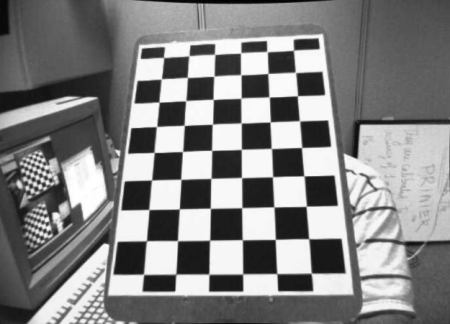
\includegraphics[width=\linewidth]{chessboard.png}
\caption{Chessboard~\cite{OpenCVCameraCalibration}}
\label{fig:chessboard}
\end{subfigure}
\hfill
\begin{subfigure}[b]{0.45\textwidth}
\centering
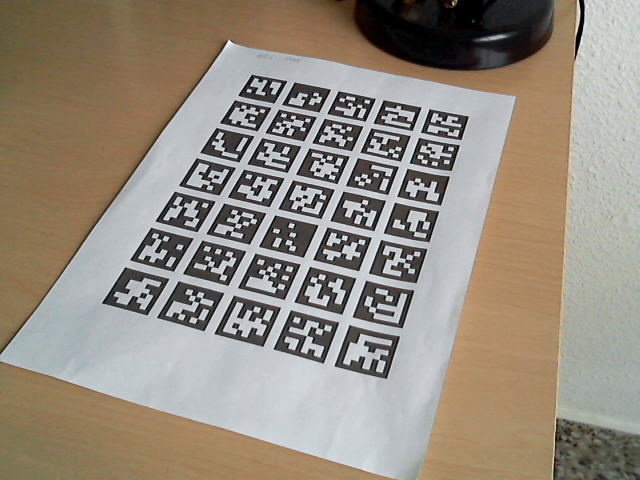
\includegraphics[width=\linewidth]{gboriginal.png}
\caption{ArUco board~\cite{OpenCVDetectionArUco}}
\label{fig:gboriginal}
\end{subfigure}
\begin{subfigure}[b]{0.45\textwidth}
\centering
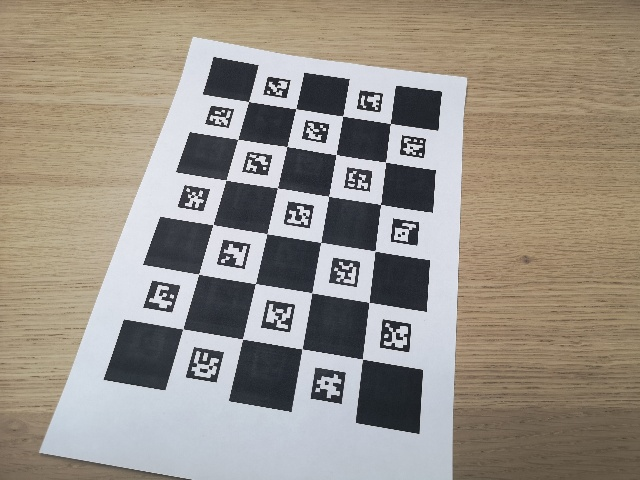
\includegraphics[width=\linewidth]{charuco.png}
\caption{Charuco board~\cite{OpenCVDetectionChArUco}}
\label{fig:charuco}
\end{subfigure}
\hfill
\begin{subfigure}[b]{0.45\textwidth}
\centering
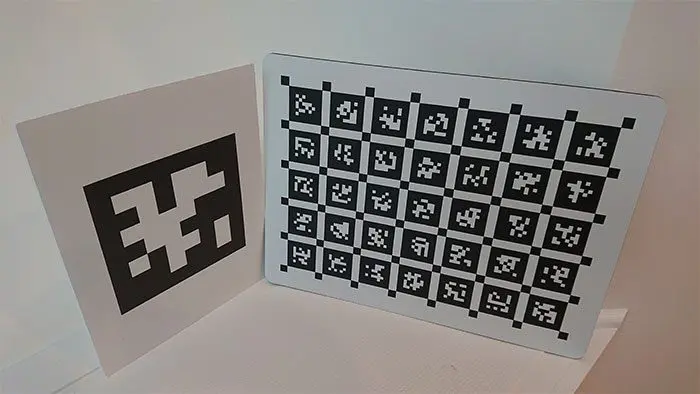
\includegraphics[width=\linewidth]{apriltag.png}
  \caption{AprilTag board~\cite{rosebrockAprilTagPython2020} (right)}
\label{fig:apriltag}
\end{subfigure}
\caption{Calibration boards.}
\end{figure}

\section{Camera models}\label{sub:camera_models}

The camera model's choice depends on the camera's physical properties
and the accuracy required. Usually, the parametric models are simpler to use, as
they have only a few parameters and deliver good accuracy. 
The most common are the Double Sphere
model~\cite{usenkoDoubleSphereCamera2018}, the Kannala-Brandt
model~\cite{kannalaGenericCameraModel2006}, and the Field-of-View
model~\cite{devernayStraightLinesHave2001}.
In the ill-posed problem of camera calibration, the common choice
of the camera model is the division
model~\cite{fitzgibbonSimultaneousLinearEstimation2001}.
However, \textcite{schopsWhyHaving102020} show that they tend to have
significantly higher errors than the non-parametric (general) models.
The \textcite{lochmanBabelCalibUniversalApproach2021} suggested a framework for
converting the parameters of a powerful back-projection
\cite{zhangFlexibleNewTechnique2000} model to recover different models' parameters.

\section{Camera parameters estimation}\label{sub:camera_parameters_estimation}

Camera calibration using repeating patterns was an important subject for a long
time, for example, \textcite{schaffalitzkyGeometricGroupingRepeated1998} in
\citeyear{schaffalitzkyGeometricGroupingRepeated1998} and
\textcite{zhangFlexibleNewTechnique2000}.

% Camera calibration is a crucial step for many computer vision tasks,
% hence many methods were proposed to solve this problem (e.g.,
% ~\cite{brownCloseRangeCameraCalibration1971},
% ~\cite{heikkilaFourstepCameraCalibration1997},
% ~\cite{fitzgibbonSimultaneousLinearEstimation2001},
% ~\cite{sturmGenericConceptCamera2004},
% ~\cite{clausRationalFunctionLens2005},
% ~\cite{meiSingleViewPoint2007},
% ~\cite{ramalingamUnifyingModelCamera2017}).

Nevertheless, camera calibration is still an open problem; recently,
multiple new approaches have arisen. 
\textcite{lochmanBabelCalibUniversalApproach2021} suggest a universal approach
to camera calibration, with a separate step of converting between camera models.
\textcite{huDeepChArUcoDark2019} used deep learning to detect ChArUcO boards.
Recently, on \citedate{duisterhofTartanCalibIterativeWideAngle2022},
\textcite{duisterhofTartanCalibIterativeWideAngle2022} introduced the iterative
approach to camera calibration, which outperforms the previous state-of-the-art
approaches for wide-angle cameras.

% The camera calibration depends a lot on the physical camera properties, choice
% of the camera model, calibration method, number of images used for calibration,
% prior knowledge of the camera, and many other variables. Therefore, currently,
% there is no established method of general camera calibration approach
% comparison, and the state-of-the-art is not well-defined. However, it is possible
% to compare the methods in the context of specific tasks and datasets.
